\chapter{Transzformerek a zene generálásnál}
\label{chap:transformers}

\section{Elméleti alapok}
\subsection{Önfigyelő mechanizmus}
Az alapművelet lekérdezéseket ($\mathbf{Q}$), kulcsokat ($\mathbf{K}$) és értékeket ($\mathbf{V}$) képez le egy kimenethez:
\[
\text{Figyelem}(\mathbf{Q},\mathbf{K},\mathbf{V}) = \text{softmax}\left(\frac{\mathbf{Q}\mathbf{K}^T}{\sqrt{d_k}}\right)\mathbf{V}
\]
ahol $d_k$ a kulcsdimenzió. Zene esetén ez lehetővé teszi tetszőleges hangjegyfüggőségek modellezését.

\subsection{Többfejű figyelem}
A párhuzamos figyelemfejek különféle kapcsolatokat rögzítenek:
\[
\text{MultiHead}(\mathbf{Q},\mathbf{K},\mathbf{V}) = \text{Concat}(\text{head}_1,...,\text{head}_h)\mathbf{W}^O
\]
Minden fej kiszámítja:
\[
\text{head}_i = \text{Figyelem}(\mathbf{Q}\mathbf{W}_i^Q, \mathbf{K}\mathbf{W}_i^K, \mathbf{V}\mathbf{W}_i^V)
\]

\section{Zene-specifikus adaptációk}
\subsection{Relatív pozíciókódolás}
A szabványos szinuszos kódolás nem működik a zenei időzítésnél. A zenei transzformer \cite{huang2018music} a következőket használja:
\[
\mathbf{A}_{i,j} = \mathbf{q}_i \mathbf{k}_j^T + \mathbf{q}_i \mathbf{r}_{i-j}^T + \mathbf{v}^T \mathbf{r}_{i-j}
\]
ahol a $\mathbf{r}$ a tanult relatív pozíció beágyazás.

\subsection{Dekódolási stratégiák}
\begin{itemize}
    \item \textbf{Autoregresszív}: Tokeneket generál balról jobbra oksági maszkolással
    \item \textbf{Nem autoregresszív}: Párhuzamos generálás iteratív finomítással
\end{itemize}

\section {Matematikai elemzés}
\subsection{Gradiens Flow}
A transzformátorok elkerülik a gradiensek eltűnését a maradék csatlakozásokon keresztül:
\[
\mathbf{h}_{l+1} = \mathbf{h}_l + \text{LayerNorm}(\text{FFN}(\text{MHA}(\mathbf{h}_l)))
\]

\subsection{Bonyolultsági szempontok}
\begin{itemize}
    \item Idő: $\mathcal{O}(T^2d)$ a $T$ sorozathosszhoz és a $d$ dimenzióhoz
    \item Memória: $\mathcal{O}(T^2)$ korlátozza a környezeti ablakot
\end{itemize}

\section{Kihívások a zenegenerációban}
\subsection{Hosszú távú függőségek}
A zenéhez több mint 100 token modellezése szükséges. Megoldások:
\begin{itemize}
    \item Memóriahatékony figyelem (pl. Reformer \cite{kitaev2020reformer})
    \item Hierarchikus modellezés (pl. szegmensszintű figyelem)
\end{itemize}

\subsection{Strukturális prioritások}
A zeneelmélet beépítése:
\begin{itemize}
    \item Harmonikus kényszerek figyelemmaszkoláson keresztül
    \item Metrikus pozíció beágyazások
\end{itemize}

\section{Zha transzformátorának megvalósítása}
\subsection{Részletek az építészetről}
A Zha Transformer egy 8 rétegű, csak dekóderhez használható architektúrát alkalmaz, amely kifejezetten zenei szekvenciák generálására optimalizált \cite{huang2018music}.

\begin{figure}[h]
\centering
\includegraphics[width=0.8\textwidth]{images/zha_transformer_arch.png}
\caption{Zha Transformer architektúra zenei generáláshoz}
\label{fig:zha_transformer}
\end{figure}

\textbf{Fő komponensek}:
\begin{itemize}
\item \textbf{8 Transformer réteg}: Optimális mélység zenei kontextushoz
\item \textbf{8 attention head}: Többféle zenei kapcsolat párhuzamos modellezése
\item \textbf{512 dimenziós embedding}: Token reprezentációs tér
\item \textbf{Pozíciós encoding}: Zenei időzítés modellezése
\item \textbf{128 input dimenzió}: MIDI hangmagasság spektrum lefedése
\end{itemize}

\subsection{Memória-alapú generálási stratégia}
A Zha Transformer innovatív memória mechanizmust alkalmaz strukturált zenei generáláshoz:

\begin{figure}[h]
\centering
\includegraphics[width=0.9\textwidth]{images/memory_mechanism.png}
\caption{Memória-alapú strukturált generálás}
\label{fig:memory_mechanism}
\end{figure}

A memória algoritmus komponensei:
\begin{enumerate}
\item \textbf{Section Memory}: Különböző zenei szakaszok (intro, verse, chorus) tárolása
\item \textbf{Context Switching}: Automatikus váltás szakaszok között
\item \textbf{Memory Retrieval}: Releváns múltbeli kontextus visszakeresése
\item \textbf{Coherence Maintenance}: Hosszú távú szerkezeti egység biztosítása
\end{enumerate}

\subsection{Structured generation algoritmus}
A Zha strukturált generálási algoritmus több fázisban működik:

\begin{figure}[h]
\centering
\includegraphics[width=0.85\textwidth]{images/structured_generation.png}
\caption{Strukturált zenei generálási folyamat}
\label{fig:structured_gen}
\end{figure}

Algoritmus lépései:
\begin{enumerate}
\item \textbf{Szakasz tervezés}: Globális struktúra (A-B-A-C forma) meghatározása
\item \textbf{Memória inicializálás}: Szakasz-specifikus memória területek létrehozása
\item \textbf{Lokális generálás}: Token-by-token generálás attention mechanizmussal
\item \textbf{Szakasz átmenetek}: Smooth váltások memória frissítéssel
\item \textbf{Globális koherencia}: Teljes kompozíció egységének ellenőrzése
\end{enumerate}

\subsection{Top-k és nucleus sampling optimalizáció}
Kifinomult sampling stratégiák a kreatív és koherens generáláshoz \cite{zhang2020deep}:

\textbf{Top-k sampling}:
\[
P_{\text{top-k}}(x_t) = \begin{cases}
\frac{P(x_t)}{\sum_{x' \in V_k} P(x')} & \text{ha } x_t \in V_k \\
0 & \text{egyébként}
\end{cases}
\]

\textbf{Nucleus (Top-p) sampling}:
\[
V_p = \text{smallest set such that } \sum_{x \in V_p} P(x) \geq p
\]

\begin{figure}[h]
\centering
\includegraphics[width=0.8\textwidth]{images/sampling_strategies.png}
\caption{Különböző sampling stratégiák összehasonlítása}
\label{fig:sampling}
\end{figure}

\subsection{JIT compilation optimalizáció}
A Zha Transformer PyTorch JIT compilation-t alkalmaz a inferencia felgyorsítására \cite{torch2023}:

A JIT optimalizáció algoritmus:
\begin{enumerate}
\item \textbf{Graph tracing}: Model execution graph rögzítése
\item \textbf{Optimization passes}: Redundáns műveletek eliminálása
\item \textbf{Kernel fusion}: GPU műveletek kombinálása
\item \textbf{Memory layout optimization}: Cache-friendly adatstruktúrák
\end{enumerate}

Teljesítmény javulások:
\begin{itemize}
\item \textbf{Inferencia sebesség}: 2-3x gyorsítás
\item \textbf{Memória hatékonyság}: 20-30\% csökkentés
\item \textbf{Batch processing}: Nagyobb throughput
\end{itemize}

\section{Esettanulmány: Bach-korálgeneráció}
\subsection{Kísérleti beállítás}
\begin{itemize}
    \item Adatkészlet: 352 korál (16 000 ütem)
    \item Bemeneti ábrázolás: Az 1. ábra a token típusokat mutatja
    \item Alaphelyzet: LSTM összehasonlítható paraméterszámmal
\end{itemize}

\centering
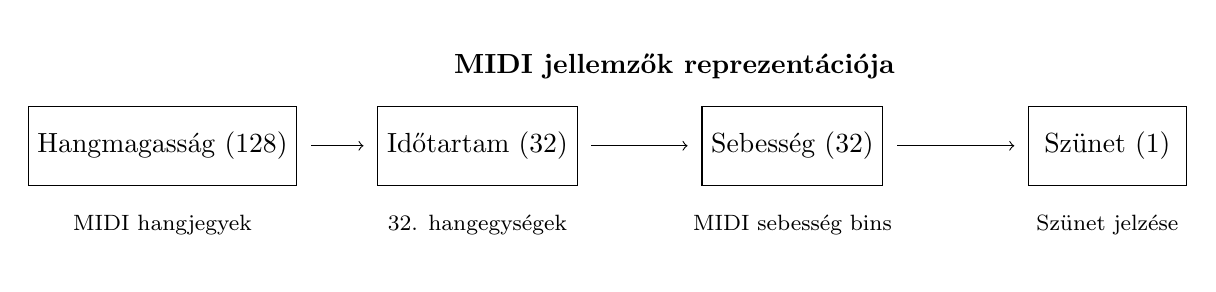
\begin{tikzpicture}[
    every node/.style={draw, minimum width=2cm, minimum height=1cm, align=center}
]

\node (pitch) at (-2,0) {Hangmagasság (128)};
\node (dur) at (2,0) {Időtartam (32)};
\node (vel) at (6,0) {Sebesség (32)};
\node (rest) at (10,0) {Szünet (1)};

\node[draw=none] at (-2,-1) {\footnotesize MIDI hangjegyek};
\node[draw=none] at (2,-1) {\footnotesize 32. hangegységek};
\node[draw=none] at (6,-1) {\footnotesize MIDI sebesség bins};
\node[draw=none] at (10,-1) {\footnotesize Szünet jelzése};

\draw[->, shorten >=5pt, shorten <=5pt] (pitch.east) -- (dur.west);
\draw[->, shorten >=5pt, shorten <=5pt] (dur.east) -- (vel.west);
\draw[->, shorten >=5pt, shorten <=5pt] (vel.east) -- (rest.west);

\node[draw=none, font=\bfseries] at (4.5,1) {MIDI jellemzők reprezentációja};

\end{tikzpicture}

\subsection{Eredmények}
\begin{table}
\centering
\begin{tabular}{lcc}
\hline
Modell és zavarodottság és motívum konzisztencia \\
\hline
LSTM és 3.2 és 0.41 \\
Transformer & \textbf{1.8} & \textbf{0.73} \\
\hline
\end{tabular}
\caption{Értékelés a Bach-korál tesztkészletről (jobb a kisebb zavarodottság)}
\end{table}

A kvalitatív elemzés kimutatta:
\begin{itemize}
    \item A transzformátorok pontos intervallumkapcsolatokkal reprodukálták a fugal alanyokat
    \item Az LSTM-ek nem tudtak 8 ütemen túl fenntartani a hangvezetési szabályokat
\end{itemize}

\section{Korlátozások és kiterjesztések}
\subsection{Főbb kihívások}
\begin{itemize}
    \item A négyzetes memória bonyolultsága korlátozza a környezetet
    \item Hidegindítási probléma üres kezdeti sorozatoknál
\end{itemize}

\subsection{Speciális változatok}
\begin{itemize}
    \item \textbf{Music Transformer}: Relatív figyelem az időzítésre
    \item \textbf{CP-Transformer}: Tanult akkordmeneti sablonok
\end{itemize}

\section{Zha Transformer implementáció részletes elemzése}
\subsection{Pozíciós kódolás implementáció}
A Zha Transformer szinuszos pozíciós kódolást használ a szekvencia pozíció információ megadásához:

\begin{lstlisting}[language=Python]
class PositionalEncoding(nn.Module):
    def __init__(self, embed_dim, max_len=2048):
        super().__init__()
        pe = torch.zeros(max_len, embed_dim)
        position = torch.arange(0, max_len, dtype=torch.float).unsqueeze(1)
        div_term = torch.exp(torch.arange(0, embed_dim, 2).float() * 
                            (-math.log(10000.0) / embed_dim))
        
        pe[:, 0::2] = torch.sin(position * div_term)
        pe[:, 1::2] = torch.cos(position * div_term)
        
        self.register_buffer('pe', pe.unsqueeze(0))
        self.dropout = nn.Dropout(0.1)
\end{lstlisting}

\subsection{Memória-alapú generálás}
A Zha Transformer innovatív memória mechanizmust implementál:

\textbf{Szakasz-alapú memória}: A modell külön memóriát tárol minden zenei szakaszhoz:
\begin{lstlisting}[language=Python]
self.section_memories = {}  # {section_id: memory_tensor}
\end{lstlisting}

\textbf{Memória frissítés}:
\begin{lstlisting}[language=Python]
def forward(self, x, use_memory=False):
    if use_memory and hasattr(self, 'memory') and self.memory is not None:
        x = torch.cat([self.memory, x], dim=1)
    
    # ... transformer processing ...
    
    if use_memory:
        max_memory_length = 1024
        self.memory = output.detach()
        if self.memory.size(1) > max_memory_length:
            self.memory = self.memory[:, -max_memory_length:, :]
\end{lstlisting}

\subsection{Strukturált generálás}
A \texttt{generate\_with\_structure} metódus összetett zenei formákat képes létrehozni:

\begin{algorithm}[H]
\SetAlgoLined
\KwIn{Seed, num\_sections, section\_length, temperature, transition\_smoothness}
\KwOut{Multi-sectional musical sequence}

Memória alaphelyzetbe állítása\;
\For{section\_id = 0 \KwTo num\_sections-1}{
    \If{section\_id in section\_memories}{
        Memória betöltése\;
    }
    \Else{
        \If{transition\_smoothness > 0}{
            Előző szakasz memóriájának keverése\;
        }
    }
    Szakasz generálása $\leftarrow$ \_generate\_section()\;
    Memória mentése section\_memories[section\_id]\;
}
Összes szakasz összefűzése\;

\caption{Strukturált generálás Zha Transformerben}
\end{algorithm}

\subsection{Sampling stratégiák}
\textbf{Top-k és Nucleus sampling kombinációja}:
\begin{lstlisting}[language=Python]
# Top-k filtering
if top_k > 0:
    indices_to_remove = next_token_logits < torch.topk(next_token_logits, top_k)[0][..., -1, None]
    next_token_logits[indices_to_remove] = -float('inf')

# Nucleus (top-p) filtering
if top_p > 0.0:
    sorted_logits, sorted_indices = torch.sort(next_token_logits, descending=True)
    cumulative_probs = torch.cumsum(F.softmax(sorted_logits, dim=-1), dim=-1)
    sorted_indices_to_remove = cumulative_probs > top_p
    # Keep first token above threshold
    sorted_indices_to_remove[..., 1:] = sorted_indices_to_remove[..., :-1].clone()
    sorted_indices_to_remove[..., 0] = 0
\end{lstlisting}

\subsection{Architektúra specifikációk}
\textbf{Modell paraméterek}:
\begin{itemize}
\item \textbf{Embedding dimenzió}: 512
\item \textbf{Figyelemfejek száma}: 8
\item \textbf{Rétegek száma}: 8
\item \textbf{Feedforward dimenzió}: 2048
\item \textbf{Dropout}: 0.1
\item \textbf{Input dimenzió}: 128 (MIDI hangmagasság spektrum)
\end{itemize}

\textbf{Batch-first konvenció}: A modell batch-first tenzor formátumot használ a hatékonyság érdekében:
\begin{lstlisting}[language=Python]
encoder_layers = nn.TransformerEncoderLayer(
    d_model=embed_dim,
    nhead=num_heads,
    dim_feedforward=dim_feedforward,
    dropout=dropout,
    batch_first=True  # [batch, seq, features]
)
\end{lstlisting}

\subsection{Optimalizálás és teljesítmény}
\textbf{JIT Compilation}: A modell JIT script formában menthető a gyorsabb inferenciához:
\begin{lstlisting}[language=Python]
try:
    scripted_model = torch.jit.script(model.cpu())
    scripted_model.save("trained_transformer_jit.pt")
    print("JIT compiled model saved for faster inference")
except Exception as e:
    print(f"JIT compilation failed: {e}")
\end{lstlisting}